\begin{ejercicio}
	Solución, expandiendo los operadores de momento angular y se utiliza la siguiente propiedad: $[AB,C] = A[B,C] + [A,C]B$.
	\begin{itemize}
		\item Demostrar $[L_x ,Y] = i\hbar Z$
			\begin{align*}
				&= [YP_z ,Y] - [ZP_y ,Y] \\
				&= Y[P_z ,Y] + [Y,Y]P_z - Z[P_z ,Y] - [Z,Y]P_y \\
				&= -Z[P_y ,Y] = -Z(-i\hbar) \\
				&= i\hbar Z.
			\end{align*}
		\item Demostrar $[L_x ,P_y] = i\hbar P_z$
			\begin{align*}
				&= [YP_z ,P_y] - [ZP_y ,P_y] \\
				&= Y[P_z ,P_y] + [Y,P_y]P_z \\
				&= i\hbar P_z.
			\end{align*}
		\item Demostrar $[L_x ,P^2] = 0$
			\begin{align*}
				&= [L_x ,P_x ^2 + P_y ^2 + P_z ^2] \\
				&= \underbrace{[YP_z,P_x ^2]}_{0} + \underbrace{[YP_z,P_y ^2]}_{2i\hbar P_y P_z} + \underbrace{[YP_z,P_z ^2]}_{0} - \underbrace{[ZP_y,P_x ^2]}_{0} - \underbrace{[ZP_y,P_y ^2]}_{0} - \underbrace{[ZP_y,P_z ^2]}_{2i\hbar P_z P_y} \\
				&= 2i\hbar [P_y,P_z] = 0
			\end{align*}
	\end{itemize}
\end{ejercicio}




\begin{ejercicio}
	Para $j=\flatfrac{3}{2}$ se tienen los posibles valores de $m = -\flatfrac{3}{2},-\flatfrac{1}{2},\flatfrac{1}{2},\flatfrac{3}{2}$. Y los ángulos de interes son $\theta _1 = \arccos{\frac{\flatfrac{3}{2}}{\flatfrac{\sqrt{15}}{2}}} = 39.2^o$ y $\theta _2 = \arccos{\frac{\flatfrac{1}{2}}{\flatfrac{\sqrt{15}}{2}}} = 75^o$. 
	
	\begin{figure}[H]
		\centering
		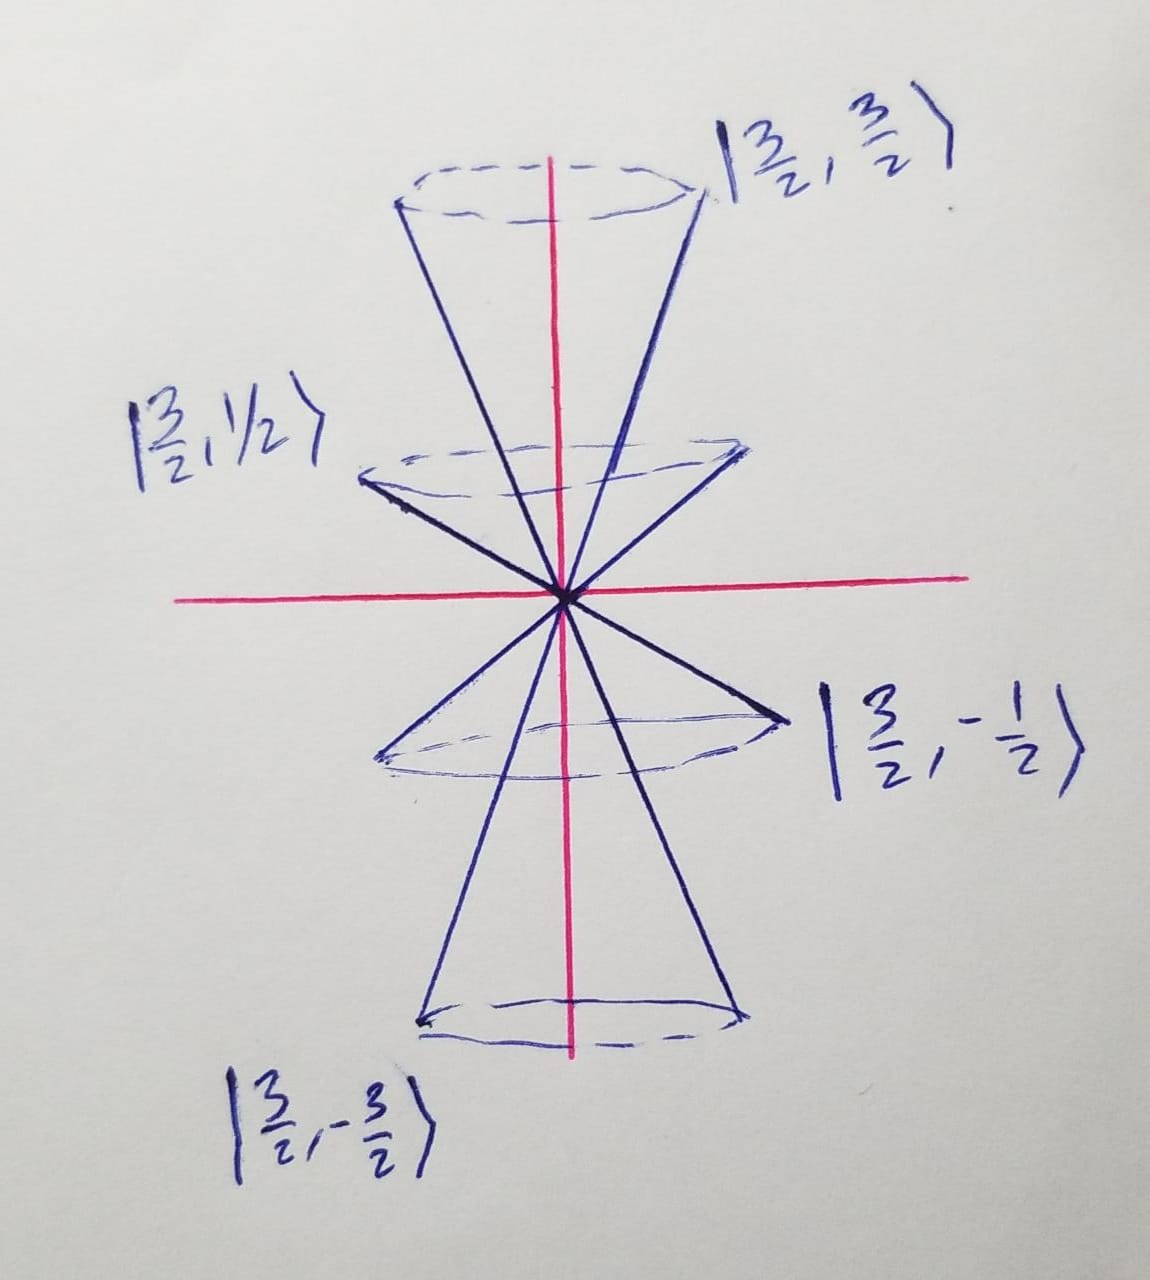
\includegraphics[scale=0.15]{img/ej2.jpeg}
		\caption{Representación de los kets propios de $J^2$.}
		\label{ej2}
	\end{figure}		
	
	También, dados los kets propios de $J^2$ y $J_z$, se tienen las entradas

		{\begin{align*}
			\begin{split}
			J^2 \ket{\frac{3}{2},-\frac{3}{2}} &= \frac{15}{4} \hbar ^2 \ket{\frac{3}{2},-\frac{3}{2}}, \\
			J^2 \ket{\frac{3}{2},-\frac{1}{2}} &= \frac{15}{4} \hbar ^2 \ket{\frac{3}{2},-\frac{1}{2}}, \\
			J^2 \ket{\frac{3}{2},\frac{1}{2}} &= \frac{15}{4} \hbar ^2 \ket{\frac{3}{2},\frac{1}{2}}, \\
			J^2 \ket{\frac{3}{2},\frac{3}{2}} &= \frac{15}{4} \hbar ^2 \ket{\frac{3}{2},\frac{3}{2}}. \\
			\end{split}
			&&
			\begin{split}
			J_z \ket{\frac{3}{2},-\frac{3}{2}} &= -\frac{3}{2} \hbar \ket{\frac{3}{2},-\frac{3}{2}}, \\
			J_z \ket{\frac{3}{2},-\frac{1}{2}} &= -\frac{1}{2} \hbar \ket{\frac{3}{2},-\frac{1}{2}}, \\
			J_z \ket{\frac{3}{2},\frac{1}{2}} &= \frac{1}{2} \hbar \ket{\frac{3}{2},\frac{1}{2}}, \\
			J_z \ket{\frac{3}{2},\frac{3}{2}} &= \frac{3}{2} \hbar \ket{\frac{3}{2},\frac{3}{2}}. \\
			\end{split}
		\end{align*}}

	Con esto, sus respectivas representaciones matriciales es
	$$ J^2 = \frac{15}{4} \hbar ^2 \mqty(1 & 0 & 0 & 0 \\ 0 & 1 & 0 & 0 \\ 0 & 0 & 1 & 0 \\ 0 & 0 & 0 & 1), $$
	$$ J_z = \frac{1}{2} \hbar \mqty(3 & 0 & 0 & 0 \\ 0 & 1 & 0 & 0 \\ 0 & 0 & -1 & 0 \\ 0 & 0 & 0 & -3). $$
	Ahora, para los operadores escaleras, se sabe que $J_\pm \ket{j,m} = \hbar\sqrt{j(j+1)-m(m\pm 1)} \ket{j,m+1}$. De la misma forma se construye la matriz para $J_+$ y para $J_- = J_+ ^\dagger$. Entonces
	$$ J_+ = \hbar \mqty(0 & 0 & 0 & 0 \\ \sqrt{3} & 0 & 0 & 0 \\ 0 & 2 & 0 & 0 \\ 0 & 0 & \sqrt{3} & 0), $$
	$$ J_- = \hbar \mqty(0 & \sqrt{3} & 0 & 0 \\ 0 & 0 & 2 & 0 \\ 0 & 0 & 0 & \sqrt{3} \\ 0 & 0 & 0 & 0). $$
	Teniendo las relaciones $J_x = \frac{1}{2} (J_+ + J_-)$ y $J_y = \frac{-i}{2} (J_+ - J_-)$, por lo que
	$$ J_x = \frac{\hbar}{2} \mqty(0 & \sqrt{3} & 0 & 0 \\ \sqrt{3} & 0 & 2 & 0 \\ 0 & 2 & 0 & \sqrt{3} \\ 0 & 0 & \sqrt{3} & 0), $$
	$$ J_y = -\frac{i\hbar}{2} \mqty(0 & -\sqrt{3} & 0 & 0 \\ \sqrt{3} & 0 & -2 & 0 \\ 0 & 2 & 0 & -\sqrt{3} \\ 0 & 0 & \sqrt{3} & 0). $$
\end{ejercicio}




\begin{ejercicio}
	Sabiendo que $L_z = -i\hbar \pdv{\phi}$, entonces, aplicando el conmutador a un vector cualquiera, se tiene
	\begin{align*}
		[L_z ,\cos{\phi} I] f &= -i\hbar \pdv{\phi} \qty(\cos{\phi} f) - \cos{\phi} \qty(-\hbar \pdv{\phi} f) \\
		&= i\hbar \sin{\phi} f - i\hbar \cos{\phi} \pdv{f}{\phi} + i\hbar \cos{\phi} \pdv{f}{\phi} \\
		&= i\hbar \sin{\phi} f;
	\end{align*}
	por ende, 
	$$ [L_z ,\cos{\phi} I] = i\hbar \sin{\phi}. $$
	Para $[L_z ,\sin{2\phi} I]$, realizamos exactamente lo mismo
	\begin{align*}
		[L_z ,\sin{2\phi} I] f &= -i\hbar \pdv{\phi} \qty(\sin{2\phi} f) - \sin{2\phi} \qty(-\hbar \pdv{\phi} f) \\
		&= -i\hbar 2\underbrace{\cos{2\phi}}_{\cos ^2 {\phi} - \sin ^2 {\phi}} f - i\hbar \sin{2\phi} \pdv{f}{\phi} + i\hbar \sin{2\phi} \pdv{f}{\phi} \\
		&= 2i\hbar \qty(\sin ^2 {\phi} - \cos ^2 {\phi}) f;
	\end{align*}
	entonces,
	$$ [L_z ,\sin{2\phi} I] = 2i\hbar \qty(\sin ^2 {\phi} - \cos ^2 {\phi}). $$
\end{ejercicio}




\begin{ejercicio}
	Sabiendo que
		$$ L^2 \ket{l,m} = \hbar ^2 l(l+1)\ket{k,m} $$
		$$ L_z \ket{l,m} = \hbar m\ket{l,m}. $$
	Ya se tiene la base propia, teniendo que $m\in [-l,l]$ entonces GRAFICA!
%	\begin{figure}[H]
%		\centering
%		\includegraphics[scale=0.5]{img/proper_basis.png}
%		\caption{Base Propia de $L^2$.}
%		\label{properbasis}
%	\end{figure}
	Además, se tiene que 
		\begin{align*}
			L_+ \ket{l,m} &= C_+ \ket{l,m} \\
			L_- \ket{l,m} &= C_- \ket{l,m},
		\end{align*}
	cuyas constantes (según Zettili) son
		\begin{align*}
			C_\pm &= \hbar \sqrt{l(l + 1) - m(m \pm 1)}.
		\end{align*}
	Encontrando las representaciones matriciales ($m' \neq m$ y $l = l' = 1$) $\mel{l,m}{\hat{A}}{l',m'}$
		\begin{align*}
			\mel{1,0}{L_-}{1,1} &= \sqrt{2} \hbar \\
			\mel{1,-1}{L_-}{1,0} &= \sqrt{2} \hbar \\
			L_- &= \frac{\hbar}{\sqrt{2}} \mqty(0 & 0 & 0 \\ 1 & 0 & 0 \\ 0 & 1 & 0)
		\end{align*}
	el resto son cero.
		\begin{align*}
			\mel{1,1}{L_+}{1,0} &= \sqrt{2} \hbar \\
			\mel{1,0}{L_+}{1,-1} &= \sqrt{2} \hbar \\
			L_+ &= \frac{\hbar}{\sqrt{2}} \mqty(0 & 1 & 0 \\ 0 & 0 & 1 \\ 0 & 0 & 0),
		\end{align*}
	$L_z$ es más claro por su definición
\begin{align*}
			\mel{1,1}{L_z}{1,1} &= \hbar \\
			\mel{1,0}{L_z}{1,0} &= 0 \\
			\mel{1,-1}{L_z}{1,-1} &= -\hbar \\
			L_z &= \hbar \mqty(1 & 0 & 0 \\ 0 & 0 & 0 \\ 0 & 0 & 1).
		\end{align*}
	Teniendo la relación entre los operadores escalera y $L_y$ y $L_x$
		$$ L_x = \frac{1}{2} \qty(L_+ + L_-), $$
		$$ L_y = \frac{i}{2} \qty(L_- - L_+). $$
	Reemplazando y sumando las matrices, se tiene
		$$ L_x = \frac{\hbar}{2\sqrt{2}} \mqty(0 & 1 & 0 \\ 1 & 0 & 1 \\ 0 & 1 & 0), $$
		$$ L_y = \frac{\hbar}{2\sqrt{2}} \mqty(0 & -1 & 0 \\ 1 & 0 & -1 \\ 0 & 1 & 0). $$
	Y $L^2 = L_x ^2 + L_y ^2 + L_z ^2$, utilizando mathematica
		$$ L^2 = \frac{\hbar ^2}{4} \mqty(5 & 0 & 0 \\ 0 & 2 & 0 \\ 0 & 0 & 4). $$
\end{ejercicio}






\begin{ejercicio}
	Sabiendo que los operadores se pueden escribir en términos del los operadores escalera
		\begin{align*}
			L_x &= \frac{1}{2} \qty(L_+ + L_-) \\
			L_y &= \frac{1}{2} \qty(L_- - L_+),
		\end{align*}
	Entonces, es claro que $\expval{L_x} = 0$ dado que $\expval{L_+} = \expval{L_-} = 0$. Ahora $L_x ^2 = \frac{1}{4} \qty(L_+ ^2 + L_+ L_- + L_- L_+ + L_- ^2)$, por lo anterior $\expval{L_+ ^2} = \expval{L_- ^2} = 0$, entonces
		$$ \expval{L_x ^2} = \frac{1}{4} \expval{L_+ L_- + L_- L_+}, $$
		$$ \expval{L_y ^2} = -\frac{1}{4} \expval{-L_+ L_- - L_- L_+}, $$
	lo que implica que $\expval{L_x ^2} = \expval{L_y ^2}$. Calculando su valor, tomamos la relación $\expval{L_x ^2} = \expval{L_y ^2} = \frac{1}{2} \qty[\expval{L^2} - \expval{L_z ^2}]$, entonces
		$$ \expval{L_x ^2} = \expval{L_y ^2} = \frac{\hbar ^2}{2} \qty[l(l + 1) - m^2]. $$
	Es claro que $l(l + 1) - m^2 \geq m(m + 1) - m^2 = m$, por ende
		$$ \Delta L_x \Delta L_y = \sqrt{\expval{L_x ^2} \expval{L_y ^2}} \geq \frac{1}{2} \hbar ^2 m. $$
\end{ejercicio}















\begin{ejercicio}
	Solución
	\begin{itemize}
		\item Para $J_+$, partimos de
			\begin{align*}
				J_z J_+ \ket{j,m} &= \qty(J_z J_+ - J_+ J_z + J_+ J_z) \ket{j,m} \\
				&= \qty([J_z ,J_+] + J_+ J_z) \ket{j,m} \\
				&= \hbar J_+ \ket{j,m} + \hbar m J_+ \ket{j,m} \\
				&= \hbar (m + 1) J_+ \ket{j,m},
			\end{align*}
		lo que implica que $J_+ \ket{j,m}$ es vector propio de $J_z$, por lo que
			$$ J_+ \ket{j,m} = C\ket{j,m + 1}. $$
		\item Para $J_-$, se tiene que
			\begin{align*}
				J_z J_- \ket{j,m} &= \qty(J_z J_- - J_- J_z + J_- J_z) \ket{j,m} \\
				&= \qty([J_z ,J_-] + J_- J_z) \ket{j,m} \\
				&= -\hbar J_- \ket{j,m} + \hbar m J_- \ket{j,m} \\
				&= \hbar (m - 1) J_- \ket{j,m},
			\end{align*}
		lo que implica que $J_- \ket{j,m}$ es vector propio de $J_z$, por lo que
			$$ J_- \ket{j,m} = C\ket{j,m - 1}. $$
	\end{itemize}
\end{ejercicio}













%%%%%